\documentclass[a4paper, 14pt]{extarticle}
\usepackage[settings]{markdown}
\usepackage{minted}

% Поля
%--------------------------------------
\usepackage{geometry}
\geometry{a4paper,tmargin=2cm,bmargin=2cm,lmargin=3cm,rmargin=1cm}
%--------------------------------------


%Russian-specific packages
%--------------------------------------
\usepackage[T2A]{fontenc}
\usepackage[utf8]{inputenc} 
\usepackage[english, main=russian]{babel}
%--------------------------------------

\usepackage{textcomp}

% Красная строка
%--------------------------------------
\usepackage{indentfirst}               
%--------------------------------------             


%Graphics
%--------------------------------------
\usepackage{graphicx}
\graphicspath{ {./images/} }
\usepackage{wrapfig}
%--------------------------------------

% Полуторный интервал
%--------------------------------------
\linespread{1.3}                    
%--------------------------------------

%Выравнивание и переносы
%--------------------------------------
% Избавляемся от переполнений
\sloppy
% Запрещаем разрыв страницы после первой строки абзаца
\clubpenalty=10000
% Запрещаем разрыв страницы после последней строки абзаца
\widowpenalty=10000
%--------------------------------------

%Списки
\usepackage{enumitem}

%Подписи
\usepackage{caption} 

%Гиперссылки
\usepackage{hyperref}

\hypersetup {
	unicode=true
}

%Рисунки
%--------------------------------------
\DeclareCaptionLabelSeparator*{emdash}{~--- }
\captionsetup[figure]{labelsep=emdash,font=onehalfspacing,position=bottom}
%--------------------------------------

\usepackage{tempora}
\usepackage{amsmath}
\usepackage{color}
\usepackage{listings}
\lstset{
  belowcaptionskip=1\baselineskip,
  breaklines=true,
  frame=L,
  xleftmargin=\parindent,
  language=Python,
  showstringspaces=false,
  basicstyle=\footnotesize\ttfamily,
  keywordstyle=\bfseries\color{blue},
  commentstyle=\itshape\color{purple},
  identifierstyle=\color{black},
  stringstyle=\color{red},
}

%--------------------------------------
%			НАЧАЛО ДОКУМЕНТА
%--------------------------------------

\begin{document}

%--------------------------------------
%			ТИТУЛЬНЫЙ ЛИСТ
%--------------------------------------
\begin{titlepage}
\thispagestyle{empty}
\newpage


%Шапка титульного листа
%--------------------------------------
\vspace*{-60pt}
\hspace{-65pt}
\begin{minipage}{0.3\textwidth}
\hspace*{-20pt}\centering

\includegraphics[width=\textwidth]{emblem}
\end{minipage}
\begin{minipage}{0.67\textwidth}\small \textbf{
\vspace*{-0.7ex}
\hspace*{-6pt}\centerline{Министерство науки и высшего образования Российской Федерации}
\vspace*{-0.7ex}
\centerline{Федеральное государственное бюджетное образовательное учреждение }
\vspace*{-0.7ex}
\centerline{высшего образования}
\vspace*{-0.7ex}
\centerline{<<Московский государственный технический университет}
\vspace*{-0.7ex}
\centerline{имени Н.Э. Баумана}
\vspace*{-0.7ex}
\centerline{(национальный исследовательский университет)>>}
\vspace*{-0.7ex}
\centerline{(МГТУ им. Н.Э. Баумана)}}
\end{minipage}
%--------------------------------------

%Полосы
%--------------------------------------
\vspace{-25pt}
\hspace{-35pt}\rule{\textwidth}{2.3pt}

\vspace*{-20.3pt}
\hspace{-35pt}\rule{\textwidth}{0.4pt}
%--------------------------------------

\vspace{1.5ex}
\hspace{-35pt} \noindent \small ФАКУЛЬТЕТ\hspace{20pt} <<Информатика, искусственный интеллект и системы управления>>

\vspace*{-16pt}
\hspace{47pt}\rule{0.83\textwidth}{0.4pt}

\vspace{0.5ex}
\hspace{-35pt} \noindent \small КАФЕДРА\hspace{50pt} <<Прикладная математика и информатика>>

\vspace*{-16pt}
\hspace{30pt}\rule{0.866\textwidth}{0.4pt}
  
\vspace{11em}

\begin{center}
\Large {\bf Лабораторная работа № 5} \\ 
\large {\bf по курсу <<Алгоритмы компьютерной графики>>}\\
% \large <<Модельно-видовые и проективные пеобразования>>
\end{center}\normalsize

\vspace{8em}


\begin{flushright}
  {Студент группы ИУ9-41Б Горбунов А. Д.\hspace*{15pt} \\
  \vspace{2ex}
  Преподаватель Цапкович П. А.\hspace*{15pt}}
\end{flushright}

\bigskip

\vfill
 

\begin{center}
\textsl{Москва 2024}
\end{center}
\end{titlepage}
%--------------------------------------
%		КОНЕЦ ТИТУЛЬНОГО ЛИСТА
%--------------------------------------

\renewcommand{\ttdefault}{pcr}

\setlength{\tabcolsep}{3pt}
\newpage
\setcounter{page}{2}

\section{Цель}\label{Sect::task}
\par
Целью работы является знакомство с  библиотекой OpenGL, принципами разработки алгоритмов копмьютерной графики и их реализацией на языке python.
\section{Задание}\label{Sect::task}
\par
а.Реализовать один из алгоритмов отсечения определенного типа в пространстве Двумерной размерности.

б. Ввод исходных данных каждого из алгоритмов производится интерактивно с помощью клавиатуры и/или мыши.

Алгоритм отсечения - отрезка произвольным многоугольником

Тип отсечения - Внешнее
\pagebreak
\section{Практическая реализация}
\begin{minted}{python}
import glfw
from OpenGL.GL import *
from math import ceil
sizeX = 1000
sizeY = 1000
data = [[255] * sizeX for i in range(sizeY)]
points = []
edges = []
cnt = 0

xmin = 200
xmax = 700
ymin = 200
ymax = 600

def key_callback(window, key, scancode, action, mods):
    global cnt, data, edges, points
    if key == glfw.KEY_SPACE and action == glfw.PRESS:
        drawLine(points[-1][0], points[-1][1], points[0][0], points[0][1])
        add_point(points[0][0], points[0][1])
    if key == glfw.KEY_1 and action == glfw.PRESS:
        miny = min([y for _, y in points])
        maxy = max([y for _, y in points])
        fill(miny + 1, maxy - 1)
    if key == glfw.KEY_2 and action == glfw.PRESS:
        filtration()
    if key == glfw.KEY_ESCAPE and action == glfw.PRESS:
        glfw.set_window_should_close(window, True)
    if key == glfw.KEY_3 and action == glfw.PRESS:
        drawLine(xmin, -ymin, xmin, -ymax)
        drawLine(xmin, -ymax, xmax, -ymax)
        drawLine(xmax, -ymax, xmax, -ymin)
        drawLine(xmax, -ymin, xmin, -ymin)
        print("drow - complite")
    if key == glfw.KEY_4 and action == glfw.PRESS:
        data = [[255] * sizeX for i in range(sizeY)]
        if len(points) > 0:
            for edge in edges:
                clip([points[edge[0]][0], points[edge[0]][1], points[edge[1]][0],  points[edge[1]][1]])
        print("Cohen-Sutherland complit")
    if key == glfw.KEY_0 and action == glfw.PRESS:
        data = [[255] * sizeX for i in range(sizeY)]
        points = []
        edges = []
        cnt = 0
        print("Clear all points")

def mouse_button_callback(window, button, action, mods):
    global cnt, data, edges, points
    if button == glfw.MOUSE_BUTTON_LEFT and action == glfw.PRESS:
        t = list(glfw.get_cursor_pos(window))
        t[0] = int(t[0])
        t[1] = int(-t[1])
        print(f"Ox = {t[0]}, Oy = {t[1]}")
        add_point(t[0], t[1])
        if len(edges) > 0:
            for edge in edges:
                drawLine(points[edge[0]][0], points[edge[0]][1], points[edge[1]][0],  points[edge[1]][1])

def add_point(x,y):
    global cnt, points
    points.append((x, y))
    cnt += 1
    add_edge()

def add_edge():
    global cnt, edges
    if cnt > 1:
        if cnt == 3:
            edges.append((0, 1)) 
        edges.append((cnt - 2, cnt - 1))

def drawLine(x0, y0, x1, y1):
    if x0 == x1:
        m = 2 ** 32
    else:
        m = ((y1 - y0) /
             (x1 - x0))
    e = -.5
    x = x0
    y = y0
    isSharp = True
    if x <= x1 and y <= y1:
        if m > 1:
            isSharp = False
            m **= -1
        while x <= x1 and y <= y1:
            data[y][x] = 0
            if isSharp:
                x += 1
            else:
                y += 1
            e += m
            if e >= 0:
                if isSharp:
                    y += 1
                else:
                    x += 1
                e -= 1
    elif x >= x1 and y <= y1:
        m = -m
        if m > 1:
            isSharp = False
            m **= -1
        while x >= x1 and y <= y1:
            data[y][x] = 0
            if isSharp:
                x -= 1
            else:
                y += 1
            e += m
            if e >= 0:
                if isSharp:
                    y += 1
                else:
                    x -= 1
                e -= 1
    elif x >= x1 and y >= y1:
        if m > 1:
            isSharp = False
            m **= -1
        while x >= x1 and y >= y1:
            data[y][x] = 0
            if isSharp:
                x -= 1
            else:
                y -= 1
            e += m
            if e >= 0:
                if isSharp:
                    y -= 1
                else:
                    x -= 1
                e -= 1
    elif x <= x1 and y >= y1:
        m = -m
        if m > 1:
            m **= -1
            isSharp = False
        while x <= x1 and y >= y1:
            data[y][x] = 0
            if isSharp:
                x += 1
            else:
                y -= 1
            e += m
            if e >= 0:
                if isSharp:
                    y -= 1
                else:
                    x += 1
                e -= 1

def filtration():
    global data
    mask = [[1, 2, 1],
            [2, 4, 2],
            [1, 2, 1]]
    for i in range(1, sizeY - 1):
        for j in range(1, sizeX - 1):
            if zeroChek(data, i, j):
                data[i][j] = int(
                    (mask[0][0] * data[i + 1][j - 1] + mask[0][1] * data[i + 1][j] + mask[0][2] * data[i + 1][j + 1] +
                     mask[1][0] * data[i][j - 1]   +   mask[1][1] * data[i][j]   +   mask[1][2] * data[i][j + 1] +
                     mask[2][0] * data[i - 1][j - 1] + mask[2][1] * data[i - 1][j] + mask[2][2] * data[i - 1][j + 1])
                    / 16)
            else:
                data[i][j] = 0
    print("filtration = True")

def zeroChek(data, i, j):
    return 0 < (data[i + 1][j - 1] + data[i + 1][j] + data[i + 1][j + 1] + data[i][j - 1] + data[i][j] + data[i][j + 1]
                + data[i - 1][j - 1] + data[i - 1][j] + data[i - 1][j + 1])

def fill(start, end): 
    global data
    for y in range(start, end):
        active_edge = []

        for edge in edges:
            x1, y1 = points[edge[0]]
            x2, y2 = points[edge[1]]
            if (y1 >= y and y2 <= y) or (y1 <= y and y2 >= y):
                dx = 1
                if (y2 - y1 != 0):
                    dx = (x2 - x1) / (y2 - y1)
                x = int(ceil(((y - y1) * dx) + x1))
                active_edge.append(x)

        active_edge.sort()
        ind, e1 = 0, 0
        for e2 in active_edge:

            if ind % 2 == 0:
                e1 = e2
            else:
                if e1 == e2:
                    ind += 1
                else:
                    for x in range(e1, e2):
                        if(data[y][x] != 0):
                            data[y][x] = 150
            ind += 1
    print("fill = True")

def sign(x):
    if x > 0:
        return 1
    else:
        return 0

#Cohen-Sutherland
def clip(mylines):
    global xmin, xmax, ymin, ymax

    bits = [0]*4
    byte = [0]*4

    x1 = mylines[0]
    y1 = -mylines[1]
    x2 = mylines[2]
    y2 = -mylines[3]

    bits[0] = sign(xmin - x1)
    byte[0] = sign(xmin - x2)
    bits[1] = sign(x1 - xmax)
    byte[1] = sign(x2 - xmax)
    bits[2] = sign(ymin - y1)
    byte[2] = sign(ymin - y2)
    bits[3] = sign(y1 - ymax)
    byte[3] = sign(y2 - ymax)

    initial = "".join(map(str, bits))
    end = "".join(map(str, byte))
    temp = ""

    if(x2 - x1 == 0):
        m = 0
    else:
        m = (y2 - y1) / (x2 - x1)
    c = y1 - m * x1
    
    print(1, end, initial, m, c)
    if initial == end and end == "0000":
        drawLine(x1, -y1, x2, -y2)
        return
    else:
        for i in range(4):
            val = bits[i] & byte[i]
            if val == 0:
                temp += '0'
            else:
                temp += '1'

        if temp != "0000":
            return

        for i in range(4):
            if bits[i] == byte[i]:
                continue
            if i == 0:
                if bits[i] == 1:
                    var = round(m * xmin + c)
                    y1 = var
                    x1 = xmin
                elif byte[i] == 1:
                    var = round(m * xmin + c)
                    y2 = var
                    x2 = xmin

            elif i == 1:
                if bits[i] == 1:
                    var = round(m * xmax + c)
                    y1 = var
                    x1 = xmax
                elif byte[i] == 1:
                    var = round(m * xmax + c)
                    y2 = var
                    x2 = xmax

            elif i == 2:
                if bits[i] == 0:
                    var = round((ymin - c) / m)
                    y1 = ymin
                    x1 = var
                elif byte[i] == 0:
                    var = round((ymin - c) / m)
                    y2 = ymin
                    x2 = var

            elif i == 3:
                if bits[i] == 1:
                    var = round((ymax - c) / m)
                    y1 = ymax
                    x1 = var
                elif byte[i] == 1:
                    var = round((ymax - c) / m)
                    y2 = ymax
                    x2 = var

        bits[0] = sign(xmin - x1)
        byte[0] = sign(xmin - x2)
        bits[1] = sign(x1 - xmax)
        byte[1] = sign(x2 - xmax)
        bits[2] = sign(ymin - y1)
        byte[2] = sign(ymin - y2)
        bits[3] = sign(y1 - ymax)
        byte[3] = sign(y2 - ymax)
        print(2, end, initial, m, c)
        if initial == end and end == "0000":
            drawLine(x1, -y1, x1, -y2)
            return
        else:
            return

def display(window):
    glClear(GL_COLOR_BUFFER_BIT | GL_DEPTH_BUFFER_BIT)
    glLoadIdentity()
    glClearColor(0, 0, 0, 0)
    glRasterPos(-1, -1)
    #glPixelZoom(2, 2)
    glDrawPixels(sizeX, sizeY, GL_LUMINANCE, GL_UNSIGNED_BYTE, data)
    glfw.swap_buffers(window)
    glfw.poll_events()
      
def main():
    if not glfw.init():
        return
    window = glfw.create_window(sizeX, sizeY, "lab_5", None, None)
    if not window:
        glfw.terminate()
        return
    glfw.make_context_current(window)
    glfw.set_key_callback(window, key_callback)
    glfw.set_mouse_button_callback(window, mouse_button_callback)
    while not glfw.window_should_close(window):
        display(window)
    glfw.destroy_window(window)
    glfw.terminate()


if __name__ == '__main__':
    main()
\end{minted}

\section{Вывод}

В данной работе я изучил возможности языка python в работе с библиотекой OpenGL, приобрёл навыки разработки на языке python алгоритмов копьютерной графики, углубил свои знания в алгоритмах отсечения. 


\section{Результат запуска}
    
\begin{figure}[!htb]
	\centering
	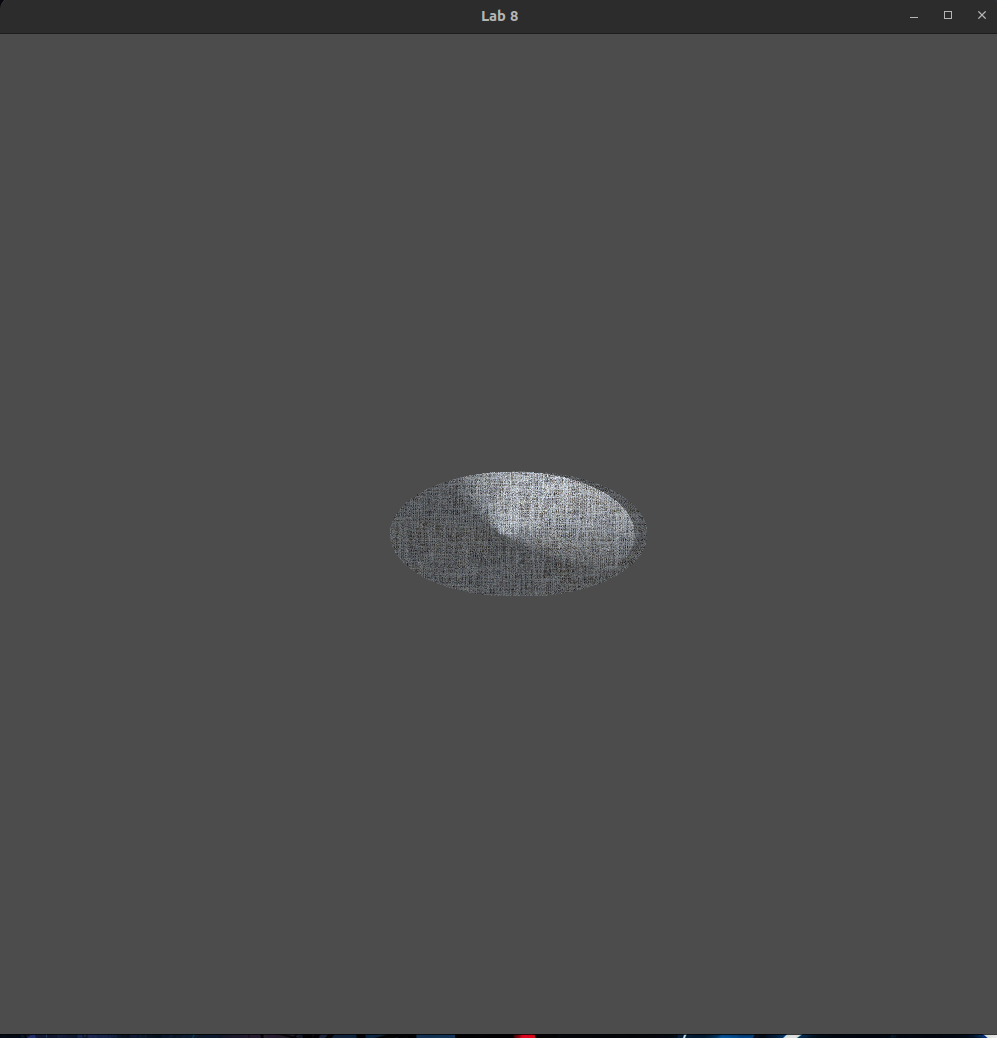
\includegraphics[width=0.8\textwidth]{picture_1.png}
\caption{До применения алгоритма отсечения}
\label{fig:picture_1.png}
\end{figure}

\begin{figure}[!htb]
	\centering
	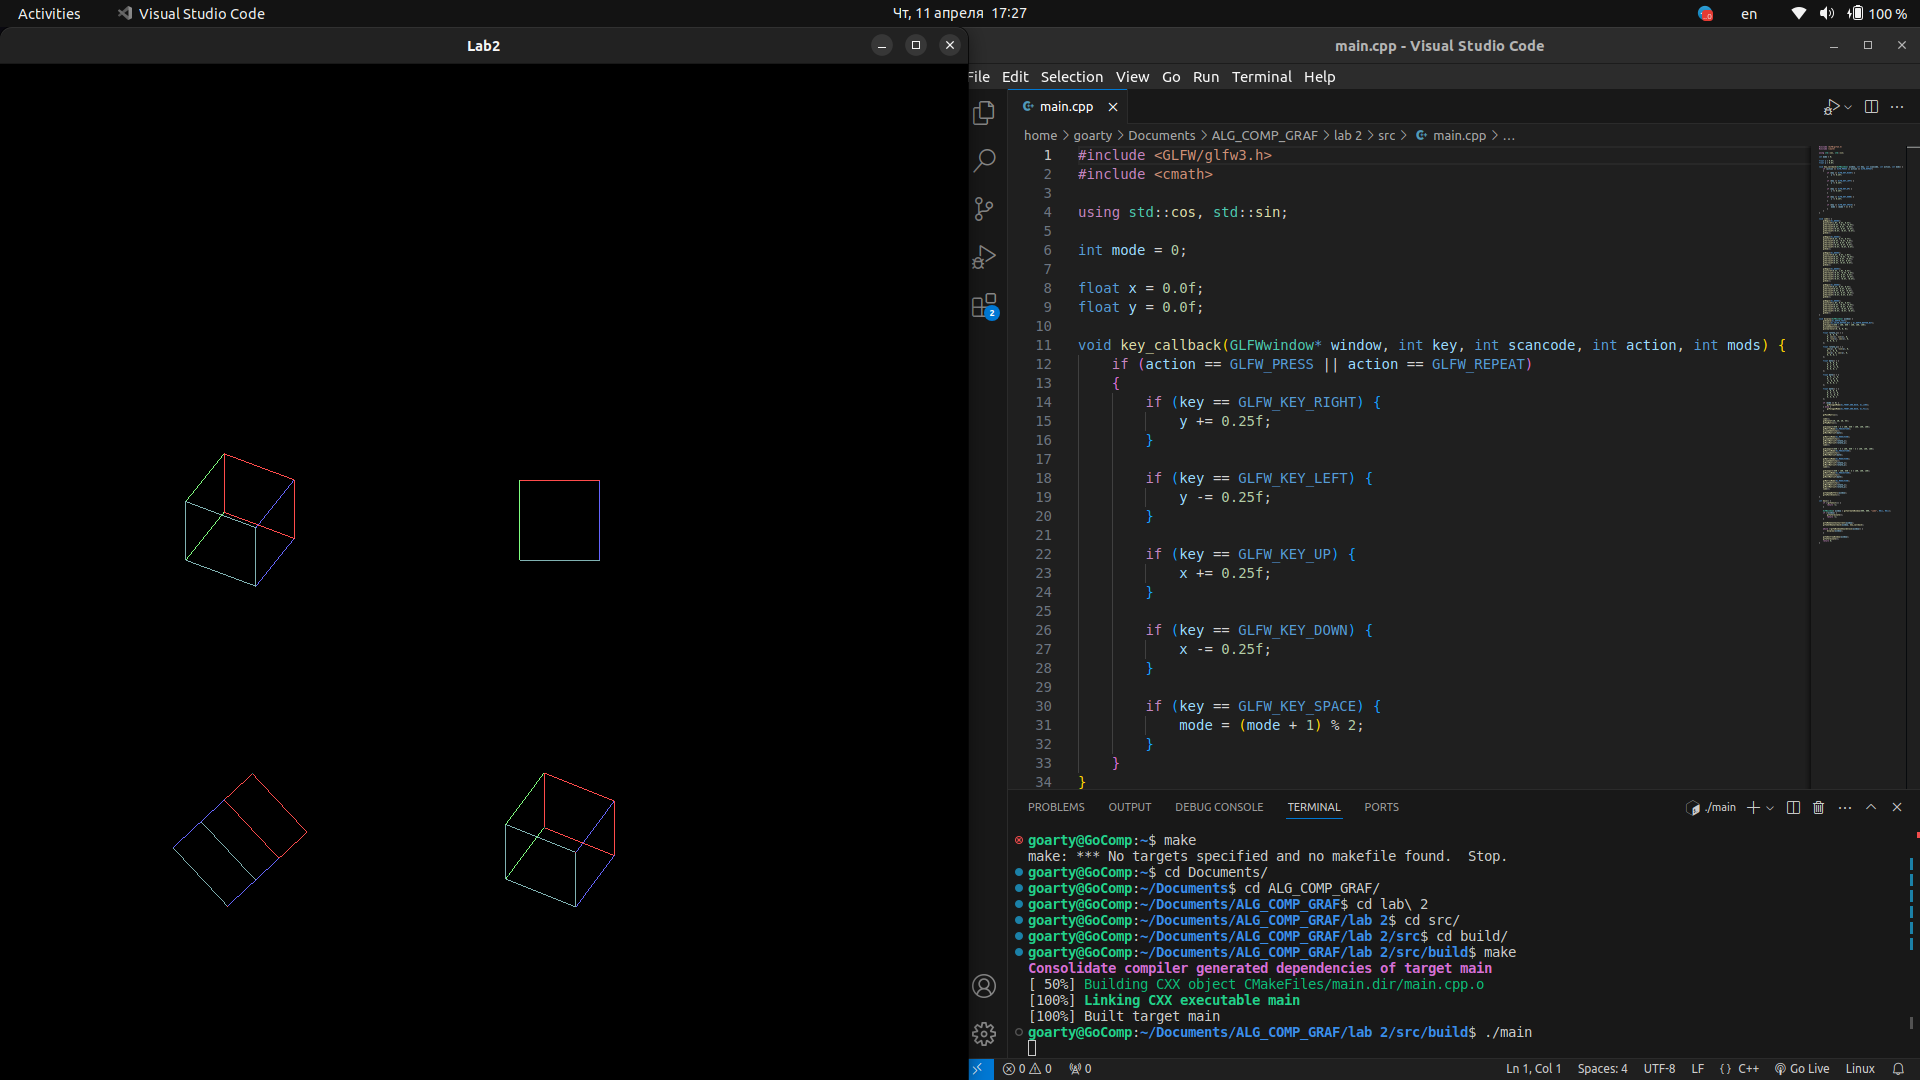
\includegraphics[width=0.8\textwidth]{picture_2.png}
\caption{После приминения алгоритма отсечения}
\label{fig:picture_2.png}
\end{figure}

\end{document}

